% t means top and the ! means to process this command right when the compiler reaches this point. 
% I had to place this here in the document so it would appear at the top of the first column rather than top of the second column and push the next figure to the next page
\begin{figure}[t!]  
	\centering
	%the command within the [] sets the width of the figure, stability-condition is the jpg name
	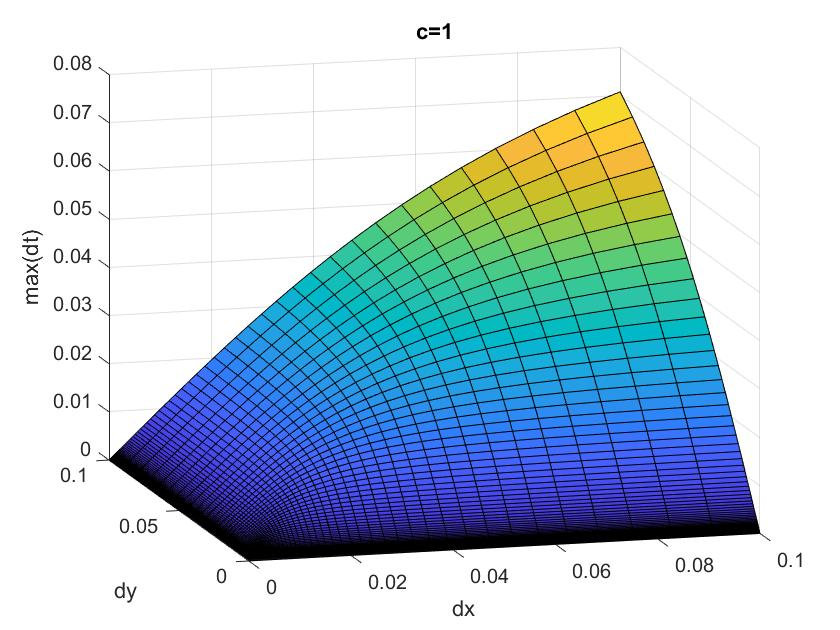
\includegraphics[width=0.9\linewidth]{stability-condition} 
	\caption{Example of caption text.}
	\label{fig:stability-condition}
\end{figure}

\section{Figures}
\label{sec:figures}
Including figures is very easy in LaTeX. It is also usually very easy to get them to appear at a desired location (e.g., the top of the page) by using simple adjustments to the figure environment. To learn more about how figures get positioned within a document (e.g., if it isn't doing what you want) you should know that they are referred to as ``floats'' in LaTeX terminology. If you google about positioning of floats in LaTeX you will likely quickly learn how you can reconfigure your TeX document to get the desired effect.

Here are some examples of how to include figures and subfigures. We can reference them like this: Fig. \ref{fig:stability-condition}, Fig. \ref{fig:waveport_ex1} is broken into two subfigures, which we can reference like Fig. \ref{subfig:waveport1} and Fig. \ref{subfig:waveport2}.

\begin{figure}[t!]
	\begin{subfigure}{0.8\linewidth} %\make this subfigure take up 80% of a linewidth
		\centering
		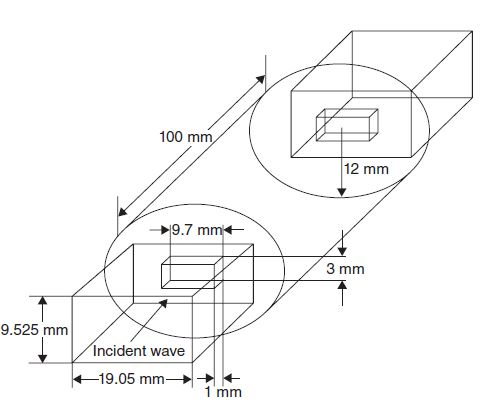
\includegraphics[width=\textwidth]{waveport1} %within this subfigure take up the entire textwidth (which was set by the linewidth command above)
		\caption{}
		\label{subfig:waveport1}
	\end{subfigure}
	\begin{subfigure}{0.9\linewidth}
		\centering
		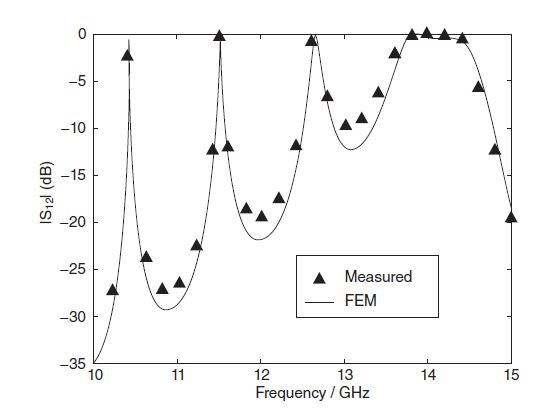
\includegraphics[width=\textwidth]{waveport2} %waveport2 is the name of the jpg file within the ./figures folder
		\caption{} %leave the caption blank, but you need the empty caption command for the (b) label to be made
		\label{subfig:waveport2}
	\end{subfigure}
	\caption{Use of wave ports to analyze a cylindrical cavity resonator. (a) The geometry analyzed and (b) the comparison of numerical and measured results (from \cite{jin2011theory}).}
	\label{fig:waveport_ex1}
\end{figure}

Here is dummy text to fill out the document to help with getting the floats positioned. The quick brown fox jumped over the lazy dog. The quick brown fox jumped over the lazy dog. The quick brown fox jumped over the lazy dog. The quick brown fox jumped over the lazy dog. The quick brown fox jumped over the lazy dog. The quick brown fox jumped over the lazy dog. The quick brown fox jumped over the lazy dog. The quick brown fox jumped over the lazy dog. The quick brown fox jumped over the lazy dog. The quick brown fox jumped over the lazy dog. The quick brown fox jumped over the lazy dog. The quick brown fox jumped over the lazy dog. The quick brown fox jumped over the lazy dog. The quick brown fox jumped over the lazy dog. The quick brown fox jumped over the lazy dog. The quick brown fox jumped over the lazy dog. The quick brown fox jumped over the lazy dog. The quick brown fox jumped over the lazy dog. The quick brown fox jumped over the lazy dog. The quick brown fox jumped over the lazy dog. The quick brown fox jumped over the lazy dog. The quick brown fox jumped over the lazy dog. The quick brown fox jumped over the lazy dog. 

